%% Lab Report for EEET2493_labreport_template.tex
%% V1.0
%% 2019/01/16
%% This is the template for a Lab report following an IEEE paper. Modified by Francisco Tovar after Michael Sheel original document.


%% This is a skeleton file demonstrating the use of IEEEtran.cls
%% (requires IEEEtran.cls version 1.8b or later) with an IEEE
%% journal paper.
%%
%% Support sites:
%% http://www.michaelshell.org/tex/ieeetran/
%% http://www.ctan.org/pkg/ieeetran
%% and
%% http://www.ieee.org/

%%*************************************************************************
%% Legal Notice:
%% This code is offered as-is without any warranty either expressed or
%% implied; without even the implied warranty of MERCHANTABILITY or
%% FITNESS FOR A PARTICULAR PURPOSE! 
%% User assumes all risk.
%% In no event shall the IEEE or any contributor to this code be liable for
%% any damages or losses, including, but not limited to, incidental,
%% consequential, or any other damages, resulting from the use or misuse
%% of any information contained here.
%%
%% All comments are the opinions of their respective authors and are not
%% necessarily endorsed by the IEEE.
%%
%% This work is distributed under the LaTeX Project Public License (LPPL)
%% ( http://www.latex-project.org/ ) version 1.3, and may be freely used,
%% distributed and modified. A copy of the LPPL, version 1.3, is included
%% in the base LaTeX documentation of all distributions of LaTeX released
%% 2003/12/01 or later.
%% Retain all contribution notices and credits.
%% ** Modified files should be clearly indicated as such, including  **
%% ** renaming them and changing author support contact information. **
%%*************************************************************************

\documentclass[journal]{IEEEtran}

% *** CITATION PACKAGES ***
\usepackage[style=ieee]{biblatex} 
\bibliography{refs.bib}

% *** MATH PACKAGES ***
\usepackage{amsmath}

% *** PDF, URL AND HYPERLINK PACKAGES ***
\usepackage{url}
% correct bad hyphenation here
\usepackage{graphicx}  % needed to include png, eps figures
\usepackage{float}  % used to fix location of images i.e. \begin{figure}[H]

\usepackage{enumitem}
\usepackage{amssymb,amsmath,amsthm, amsfonts}
\usepackage[all]{xy} % for diagrams with arrows
\usepackage{tikz-cd} % for diagrams with arrows
\usepackage{graphicx} % to manage images

% Sections (theorems, propositions, lemmas…) =====================================================================================================================
\newtheorem{theorem}{Theorem}[section]
\newtheorem{lemma}[theorem]{Lemma}
\newtheorem{corollary}[theorem]{Corollary}
\newtheorem*{conjecture}{\bf Conjecture}
\newtheorem{proposition}[theorem]{Proposition}
% \numberwithin{theorem}{section} % To display the section number in the theorem

\theoremstyle{definition}
\newtheorem{definition}[theorem]{Definition}
\newtheorem{assumption}[theorem]{Assumption}
\newtheorem{exercise}{Exercise}
\newtheorem*{solution}{Solution}
\newtheorem*{answer}{Answer}
\newtheorem*{claim}{Claim}

\theoremstyle{remark}
\newtheorem*{theoremno}{{\bf Theorem}}
\newtheorem*{remark}{Remark}
\newtheorem*{example}{Example}
\newtheorem*{hint}{Hint}



% Commands =====================================================================================================================
\def\bb#1{\mathbb{#1}}
\def\cal#1{\mathcal{#1}}
\def\frak#1{\mathfrak{#1}}
\def\rm#1{\mathrm{#1}}
\def\bf#1{\mathbf{#1}}
\newcommand{\C}{\mathbb{C}}
\newcommand{\R}{\mathbb{R}}
\newcommand{\N}{\mathbb{N}}
\newcommand{\Z}{\mathbb{Z}}
\newcommand{\Q}{\mathbb{Q}}
\newcommand{\K}{\mathbb{K}}
\newcommand{\bbP}{\mathbb{P}}
\newcommand{\F}{\mathcal{F}}
\newcommand{\calP}{\mathcal{P}}
\newcommand{\G}{\mathcal{G}}
\newcommand{\calL}{\mathcal{L}}
\newcommand{\calC}{\mathcal{C}}
\newcommand{\calN}{\mathcal{N}}
\newcommand{\calF}{\mathcal{F}}
\newcommand{\calE}{\mathcal{E}}
\newcommand{\frakA}{\mathfrak{A}}
\newcommand{\frakS}{\mathfrak{S}}
\newcommand{\esp}{\mathbb{E}}
% \P = caracs spéciaux,\S = paragraphe, \L = L barre

% Existe déjà : ker, partie Im, Re, min, max, inf, sup, log, exp, sin, sinh, cos, cosh,, tan lim, liminf, limsup
\DeclareMathOperator{\Id}{Id}
\DeclareMathOperator{\Hom}{Hom}
\DeclareMathOperator{\Ima}{Im}
\DeclareMathOperator{\Homeo}{Homeo}
\DeclareMathOperator{\Aut}{Aut}
\DeclareMathOperator{\Bij}{Bij}
\DeclareMathOperator{\Isom}{Isom}
\DeclareMathOperator{\GL}{GL}
\DeclareMathOperator{\End}{End}
\DeclareMathOperator{\rang}{rang}
\DeclareMathOperator{\rank}{rank}
\DeclareMathOperator{\vol}{vol}
\DeclareMathOperator{\sgn}{sgn}
\DeclareMathOperator{\var}{Var}
\DeclareMathOperator{\erf}{erf}
\DeclareMathOperator{\spec}{spec}
\DeclareMathOperator{\diag}{diag}
\DeclareMathOperator{\pgcd}{pgcd}
\DeclareMathOperator{\pgdc}{pgdc}

% Lois de probabilités
\DeclareMathOperator{\Geom}{Geom}
\DeclareMathOperator{\Bin}{Bin}
\DeclareMathOperator{\Exp}{Exp}
\DeclareMathOperator{\Ber}{Ber}
\DeclareMathOperator{\Student}{Student}
\DeclareMathOperator{\Poi}{Poi}
\newcommand{\czero}{\calC^0}
\newcommand{\cone}{\calC^1}
\newcommand{\ctwo}{\calC^2}
\newcommand{\cinf}{\calC^{\infty}}
\newcommand{\bigpeter}[1]{\Big\langle#1\Big\rangle}
\newcommand{\peter}[1]{\langle#1\rangle}
\newcommand{\transp}[1]{#1^t}
\newcommand{\series}[2]{\sum_{#1}^{\infty}#2}
\newcommand{\intt}[4]{\int_{#1}^{#2}#3\mathrm{d}#4}
\newcommand{\ddt}[1]{\frac{\mathrm{d}#1}{\mathrm{dt}}}
\newcommand{\deldt}[1]{\frac{\partial#1}{\partial\mathrm{t}}}
\newcommand{\rmd}[1]{\mathrm{d}#1}
\newcommand{\inv}[1]{#1^{-1}}
\newcommand{\dx}{\rmd x}
\newcommand{\dy}{\rmd y}
\newcommand{\dz}{\rmd z}
\newcommand{\dt}{\rmd t}
\newcommand{\du}{\rmd u}
\newcommand{\dv}{\rmd v}
\newcommand{\ds}{\rmd s}
\newcommand{\dxy}{\rmd xy}
\newcommand{\dyz}{\rmd yz}
\newcommand{\dyx}{\rmd yx}
\newcommand{\dzy}{\rmd zy}
\newcommand{\dzx}{\rmd zx}
\newcommand{\dxz}{\rmd xz}
\newcommand{\gtinf}[1]{\underset{#1\to\infty}{\longrightarrow}}
\newcommand{\sm}[4]{\begin{psmallmatrix}#1&#2\\#3&#4\end{psmallmatrix}}
\newcommand{\map}[4]{
	\begin{matrix}
		#1&\to&#2\\#3&\mapsto&#4
	\end{matrix}
}



\begin{document}

% paper title
\title{Study of the properties of the Relaxed Recentered Log-Barrier function based Nonlinear Model Predictive Control (RRLB NMPC)}

% author names 
\author{Tudor Oancea}% <-this % stops a space
        

% make the title area
\maketitle

% As a general rule, do not put math, special symbols or citations
% in the abstract or keywords.
\begin{abstract}
    Hello
\end{abstract}

\section{Introduction}
Include a title and one or two paragraphs describing what you plan to do.
Tell what interviews, site visits, or other activity you plan.
Be specific if you can.
Include  one good reference you plan to used. This is an example of how to include a citation.

\section{Background}
Give a background on your topic. Include references. 

\section{The RRLB MPC}\label{sec:RRLB-MPC}
\begin{align}
	\begin{split}
		\label{eq:NMPC}
		V_N(x)=\underset{\bf{x},\bf{u}}{\min} &\quad \sum_{k=0}^{N-1}l(x_k,u_k)~+~F(x_N)\\
		\text{s.t.} &\quad x_0=x\text{ and }x_{k+1}=f(x_k,u_k),~k=0,\ldots,N-1\\
		&\quad x_k\in\cal{X},~k=0,\ldots,N\\
		&\quad u_k\in\cal{U},~k=0,\ldots,N-1
	\end{split}
\end{align}

In this section we will introduce the RRLB functions, formulate the RRLB MPC and recall the results proved in the linear case in \cite{RRLB-linear-MPC}.
As mentioned in the last section, we will suppose that $x^*=0\in\cal{X}^\circ$ and $u^*=0\in\cal{U}^\circ$.

Before introducing the RRLB MPC, let's first state the principal problem it solves.
In practice, it might happen than the constraints are violated because of external disturbances or because of the presence of \textit{model mismatch}, i.e. the system's evolution is not perfectly described by the dynamics used in the MPC.
In this case, the NLP defining the MPC~\ref{eq:NMPC} becomes unfeasible and the algorithm implementing it will either crash or return solutions that are not optimal at all.
A common way to fix such problem is to use \textit{soft constraints} on the state and control constraints, by introducing \textit{slack parameters} that are penalized in the objective function.
Such approaches were reported for example in \cite{soft-constrained-MPC}.
The problem with soft-constrained formulations is the incapacity of providing closed-loop properties like asymptotic stability or constraints satisfaction, unless nonsmooth penalty functions are used, which dramatically impacts the performance of algorithms in charge of solving the NLP.
RRLB functions are designed to overcome this limitations while still preserving the recursive feasibility properties.

\vspace{12pt}

Let's first take a step back and recall what regular log-barrier functions are.
We will only give the definitions for the states $x\in\R^{n_x}$, since they only depend on the nature of the constraint set and not on the actual quantity represented.

For a simple constraint of the form $c^Tx\leq d$, the associated \textit{log-barrier function} is defined as $-\log(d-c^Tx)$.
Such a function is defined on the interior of the feasible set of the constraint and becomes infinity near its boundary.
For a set of polytopic constraints $\left\{ x~|~C_xx\leq d_x \right\}$, we can define the log-barrier as the sum of the log-barriers for each constraint:
$$B_x(x)=\sum_{i=1}^{q_x}-\log(d_{x,i}-\rm{row}_i(C_x)x)$$
where $q_x$ is the number of constraints, or equivalently the numbers of rows in $C_x$\,.

A first interesting property we would like to add to our log-barrier function is the one of \textit{positive definiteness}, i.e. $B_x(x)>0,~\forall x\neq 0$ in a neighborhood of the origin.
To this end we introduce the notion of \textit{weight recentered log-barrier function} as defined in \cite{RLB}:
$$B_x(x)=\sum_{i=1}^{q_x}(1+w_{x,i})\left[\log(d_{x,i})-\log(d_{x,i}-\rm{row}_i(C_x)x)\right]$$
where the weights $w_{x,i}$ are chosen such that $B_x(0)=0$ and $\nabla B_x(0)=0$.
It is shown in \cite{RLB} that such weights always exist when the constraint set is polytopic (i.e. polyhedral and bounded) and that weight-recentered log-barrier functions are positive definite and upper-bounded by a quadratic.

The second important property we have to add is the definiteness on the whole space.
For a given \textit{relaxation parameter} $\delta>0$, we can define the \textit{relaxed recentered log-barrier function}, or \textit{RRLB} function as follows:
\begin{align*}
	B_x(x)&=\sum_{i=1}^{q_x}(1+w_{x,i})B_{x,i}(x)\\
	\text{ with }B_{x,i}(x)&=\begin{cases}
		\log(d_{x,i})-\log(d_{x,i}-\rm{row}_i(C_x)x)&\text{if }d_{x,i}-\rm{row}_i(C_x)x>\delta\\
		\beta(d_{x,i}-\rm{row}_i(C_x)x;\delta)&\text{ otherwise}
	\end{cases}
\end{align*}
where $\beta$ is a twice continuously function that extends the log-barrier to a twice continuously differentiable function on $\R$.
The simplest example of such a function is
$$\beta(z;\delta)=\frac{1}{2}\left[ \left( \frac{z-2\delta}{\delta} \right)^2-1 \right]-\log(\delta)$$
To ensure that this function still verifies $B_x(0)=0$ and $\nabla B_x(0)=0$, we need to choose $0<\delta\leq\min\left\{d_{x,1},\ldots,d_{x,q_x},d_{u,1},\ldots,d_{u,q_u}\right\}$\,, which is always possible if $0\in\cal{X}$ and $0\in\cal{U}$\,.
An illustration of this relaxation procedure can be found in figure~\ref{fig:RRLB-functions} found in \cite{rti-diehl}.

\begin{figure}
	\centering
	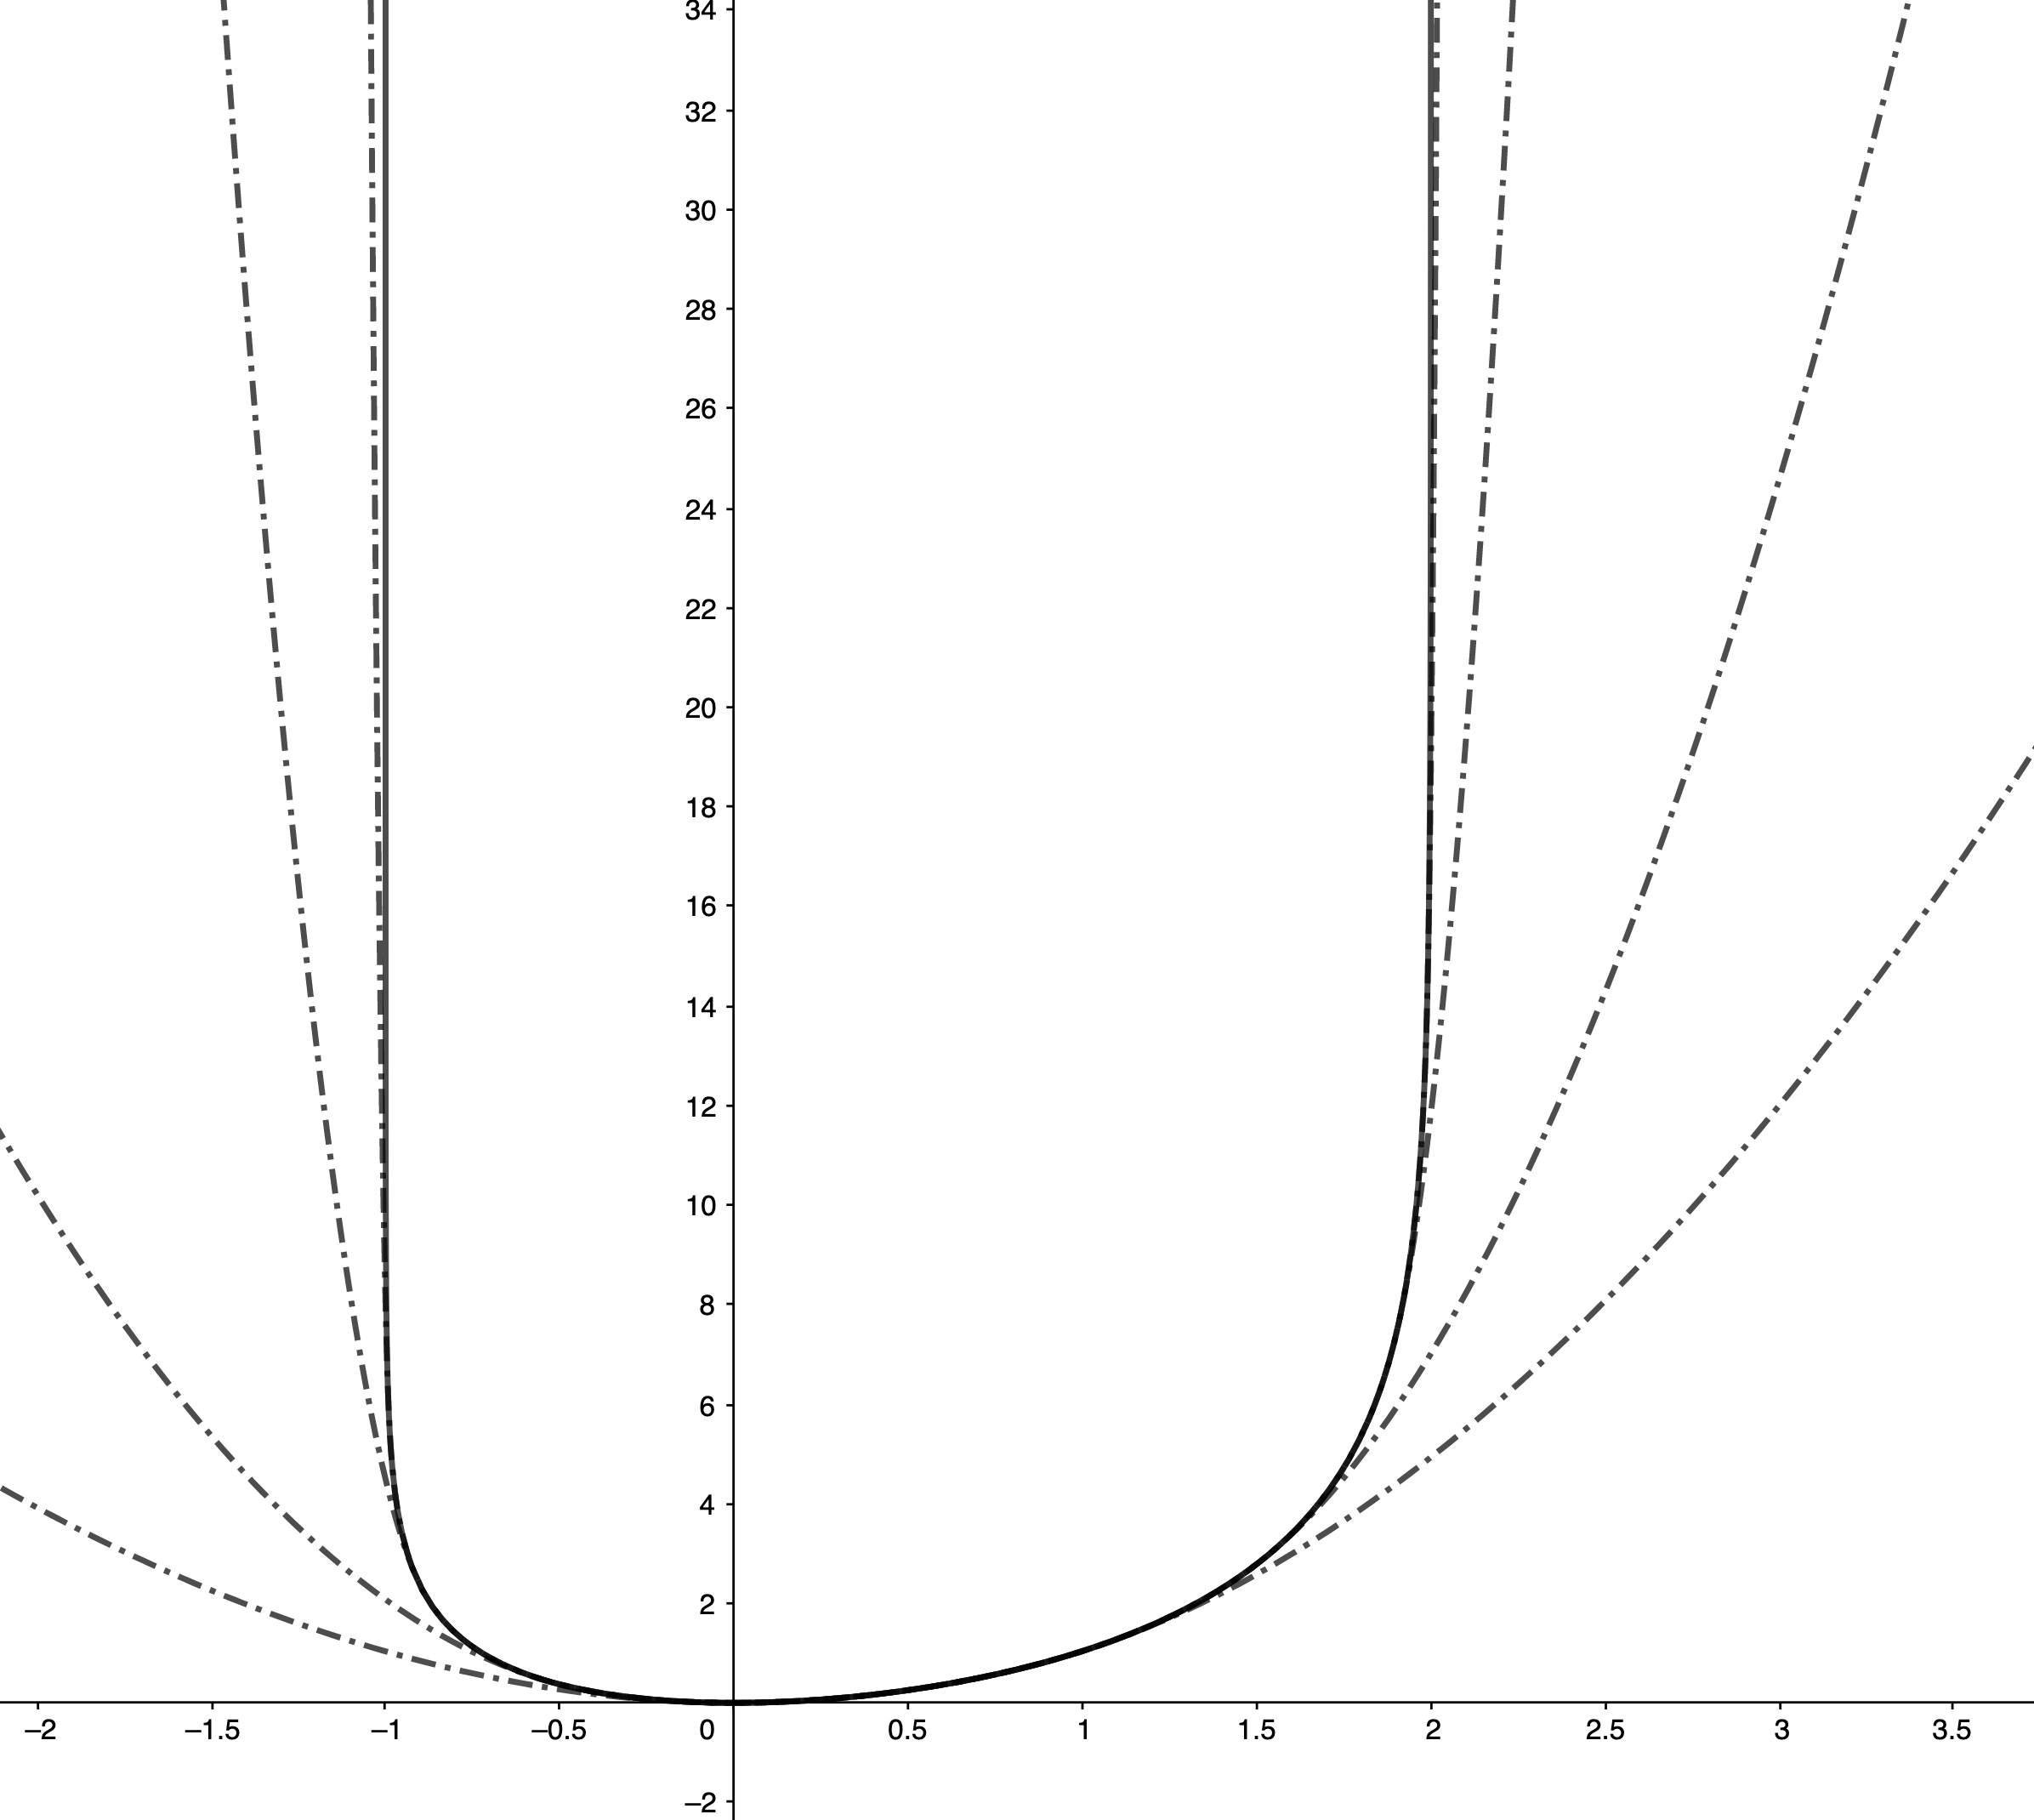
\includegraphics[width=0.5\textwidth]{images/rrlb-functions.png}
	\caption{\textit{(Left)}: Principle of relaxed log barrier function based on quadratic relaxation. (\textit{Right}): Regular weight recentered log barrier function (solid line) and RRLB function for $\delta\in\left\{ 0.01,0.1,0.5,1 \right\}$ for the constraint $z\in\R,~-1\leq z\leq 2$}
	\label{fig:RRLB-functions}
\end{figure}

\vspace{24pt}

\noindent With all these definitions we can finally define the \textit{RRLB MPC}:
\begin{align}
	\begin{split}\label{eq:RRLB-NMPC}
		\tilde{V}_N(x)=\underset{\bf{x},\bf{u}}{\min} &\quad \tilde{J}_N(\bf{x},\bf{u})\\
		\text{s.t.} &\quad x_0=x\text{ and }x_{k+1}=f(x_k,u_k),~k=0,\ldots,N-1\\
	\end{split}
\end{align}
where the new objective function $\tilde{J}_N(\bf{x},\bf{u})=\sum_{k=0}^{N-1}\tilde{l}(x_k,u_k)~+~\tilde{F}(x_N)$ is defined using the new stage costs $\tilde{l}(x,u)=l(x,u)+\epsilon B_x(x)+\epsilon B_u(u)$ and the new terminal cost $\tilde{F}(x)=x^TPx$ for another matrix $P$ that will be determined in such a way that the control law given by the MPC yields an asymptotically stable system.
The barrier parameter $\epsilon$ has in theory the following interpretation: when it goes to zero, the solution of problem~\ref{eq:RRLB-NMPC} converges to the one of~\ref{eq:NMPC}.
However, we will here consider it as fixed for simplicity.

\vspace{12pt}

\noindent When we consider the RRLB MPC~\ref{eq:RRLB-NMPC} in the case of linear dynamics $x^+=Ax+Bu$, we know the two following theorems to be true:

\begin{theorem}[Theorem 5 in \cite{RRLB-linear-MPC}]
	\label{nominal-stability-linear-case}
	Suppose that the pair $(A,B)$ is stabilizable and that the matrix $P$ is chosen as the unique positive definite solution to the following modified DARE:
	$$P=A^TPA-A^TPB(R+\epsilon M_u+B^TPB)^{-1}B^TPA+Q+\epsilon M_x$$
	where $M_x=\nabla^2 B_x(0)$ and $M_u=\nabla^2 B_u(0)$\, are the hessian of the RRLB functions at the origin.

	Then for any initial state $x(0)\in\R^{n_x}$, the control law given by the MPC yields an asymptotically stable system.
\end{theorem}

\begin{theorem}[Lemma 5 in \cite{RRLB-linear-MPC}]
	\label{constraint-satisfaction-guarantee-linear-case}
	In the same conditions as in the previous theorem, there is a neighborhood $\cal{X}_N(\delta)$ of the origin such that for any initial state $x(0)\in\cal{X}_N(\delta)$, all the constraint will be satisfied along the closed-loop trajectories.
	Furthermore, the set $\cal{X}_N(\delta)$ is given explicitly by:
	$$\cal{X}_N(\delta)=\left\{x\in\cal{X}~|~\tilde{V}_N(x(0))-x(0)^TP_{\rm{LQR}}x(0)\leq\min\{\beta_x(\delta),\beta_u(\delta)\}\right\}$$
	where $P_{\rm{LQR}}$ is the solution to the classical DARE and
	$$\beta_x(\delta)=\underset{i,x}{\min}\left\{ B_x(x)~|~\rm{row}_i(C_xx)=d_{x,i} \right\},\quad \beta_u(\delta)=\underset{i,u}{\min}\left\{ B_u(u)~|~\rm{row}_i(C_uu)=d_{u,i} \right\}$$
\end{theorem}

\noindent Additional results were proven in the linear case, such as the existence of a procedure to find $\delta$ such that the maximum constraint violation along the closed-loop trajectories is bounded by a pre-defined tolerance.
In the nonlinear case, however, we will not be able to prove such powerful results because of the lack of knowledge on the error terms that appear in the dynamics (see subsection~\ref{sec:constraints-satisfaction-guarantees}).

\section{Theoretical properties of RRLB Nonlinear MPC}\label{sec:RRLB-theoretical-properties}

In this section, we consider the RRLB MPC~\ref{eq:RRLB-NMPC} with nonlinear dynamics and show that the results of the previous section hold locally, in a neighborhood of the origin.

From this point on, for an initial state $x\in\R^{n_x}$ we will denote by \newline
$\tilde{\bf{x}}(x)=\left\{ \tilde{x}_0(x)=x,\tilde{x}_1(x),\ldots,\tilde{x}_N(x) \right\}$ and $\tilde{\bf{u}}(x)=\left\{ \tilde{u}_0(x),\tilde{u}_1(x),\ldots,\tilde{u}_{N-1}(x) \right\}$ the optimal sequences of states and controls found by the RRLB MPC.
When no confusion is possible we will drop the "$(x)$".

\subsection{Nominal asymptotic stability}\label{sec:RRLB-nominal-stability}

\begin{lemma}
	\label{thm:Lipschitzianity}
	Consider the RRLB MPC~\ref{eq:RRLB-NMPC} and re-write it in a simpler way as
	$$\tilde{V}_N(x)=\underset{\bf{u}}{\min} \quad J(x,\bf{u})$$
	where $J(x,\bf{u})=\tilde{l}(x,u_0)+\tilde{l}(f(x,u_0),u_1)+\cdots+\tilde{F}(f(f(...),u_{N-1}))$\,.
	If for a certain initial state $\bar{x}$ we suppose that $D_\bf{u}J(\bar{x},\tilde{\bf{u}})=0$ and $\nabla_{\bf{u}\bf{u}}^2J(\bar{x}, \tilde{\bf{u}})\succ 0$ (the matrix is positive definite) then in a neighborhood of $\bar{x}$ we have:
	\begin{itemize}[label=\textbullet]
		\item $\forall k=0,\ldots,N-1,\quad \|\tilde{u}_k(x)\|=O(\|x\|)$
		\item $\forall k=1,\ldots,N,\quad \|\tilde{x}_k(x)\|=f(f(\ldots,u_{k-2}),u_{k-1})=O(\|x\|)$
	\end{itemize}
\end{lemma}
\begin{proof}
	We can use the proof of the Theorem 4.2 in \cite{lectures-parametric-optimization} to argue that each $\tilde{x}_k$ and $\tilde{u}_k$ is continuously differentiable in a closed neighborhood of the origin.
	Therefore, by continuity their gradient is bounded on this neighborhood and they are Lipschitz.
\end{proof}

\noindent Now our main result:

\begin{theorem}\label{thm:nominal-stability}
	Let's consider the problem~\ref{eq:RRLB-NMPC} and assume the following:
	\begin{enumerate}
		\item If we denote the objective function as $J(x,\bf{u})$ as in Lemma~\ref{thm:Lipschitzianity}, we have $D_\bf{u}J(0,\bf{u}(0))=D_\bf{u}J(0,0)=0$ and $\nabla^2_{\bf{u}\bf{u}}J(0,\bf{u}(0))=\nabla^2_{\bf{u}\bf{u}}J(0,0)\succ 0$

		\item When linearizing the system dynamics around the origin and letting $A=D_xf(0,0),$ $B=D_uf(0,0)$, we suppose that the pair $(A,B)$ is stabilizable.
		This implies in particular that there exists a stabilizing cost $K$, i.e. a matrix such that $A_K:=A+BK$ only has eigenvalues in the unit disk.

		\item The matrix $P$ defining the terminal costs is the unique positive definite solution to the following Lyapunov equation:
		\begin{equation*}
			P=A_K^TPA_K+\mu Q_K
		\end{equation*}
		where $\mu>1$ and $Q_K=Q+\epsilon M_x+K^T(R+\epsilon M_u)K$\,.
	\end{enumerate}
	Then the dynamical system $x^+=f(x,\tilde{u}_0(x))$ is LAS, i.e. for all initial state in a neighborhood of the origin, the control law given by the RRLB MPC yields an asymptotically stable system.
\end{theorem}

\begin{remark}~
	The matrix $K$ can be constructed using the DARE for the following modified infinite horizon LQR problem:
	\begin{align}
		\begin{split}\label{eq:inf-LQR}
			\underset{\bf{x},\bf{u}}{\min} &\quad \sum_{k=0}^\infty x_k^T(Q+\epsilon M_x)x_k+u_k^T(R+\epsilon M_u)u_k\\
			\text{s.t.} &\quad x_{k+1}=Ax_k+Bu_k,~k=0,\ldots,N-1\\
		\end{split}
	\end{align}
	where $M_x=\nabla^2B_x(0)$ and $M_u=\nabla^2B_u(0)$, i.e.
	$$\begin{cases}
		K=-(R+B^T\Pi B)^{-1}B^T\Pi A&\\
		\Pi=A_K^T\Pi A_K+Q_K
	\end{cases}$$
	The only difference between this last equation and the Lyapunov equation in the statement of the theorem is the $\mu$ term.
	In theory it is very important, but in practice, we can actually take it very close to 1 and find $P$ and $K$ by solving
	$$\begin{cases}
		K=-(R+B^TP B)^{-1}B^TP A&\\
		P=A_K^TP A_K+Q_K
	\end{cases}$$
	% This is what we will do in section~\ref{sec:RRLB-numerical-experiments}.
\end{remark}

\begin{proof}~
	To prove the result we will show that $\tilde{V}_N$ is a Lyapunov function in a neighborhood of the origin.
	First, using the recentering of the RRLB functions, we can write the Taylor expansion of the stage costs $\tilde{l}$:
	\begin{align*}
		\tilde{l}(x,u)&=x^T[\nabla_{xx}^2\tilde{l}(0,0)] x+u^T[\nabla_{uu}^2\tilde{l}(0,0)]u+O(\|x\|^3+\|u\|^3)\\
		&=x^T[Q+\epsilon M_x]x+u^T[R+\epsilon M_u]u+O(\|x\|^3+\|u\|^3)\\
		\implies\tilde{l}(x,Kx)&=x^TQ_Kx+O(\|x\|^3)\,.
	\end{align*}
	By the second assumption, we also have $\forall x\in\R^{n_x}$:
	We can use the same reasoning as in the paragraph 2.5.5 of \cite{MPC-book} to show that $\tilde{F}$ is a local Lyapunov function, i.e. there exists a neighborhood of the origin in which:
	$$\tilde{F}(A_Kx)+\mu x^T Q_K x-\tilde{F}(x)=0$$
	$$\tilde{F}(f(x,Kx))+x^T Q_K x-\tilde{F}(x)\leq 0\Longrightarrow\tilde{F}(f(x,Kx))-\tilde{F}(x)+\tilde{l}(x,Kx)=O(\|x\|^3)\,.$$

	\noindent What's more, by previous lemma, the predicted states are all Lipschitz with respect to the initial state, so we can choose an even smaller neighborhood such that $\tilde{x}_N(x)$ is also in it.

	\noindent Now using the optimal sequence of states and controls of the RRLB MPC starting at $x$, we can construct new feasible sequences for the problem starting at $\tilde{x}_1(x)$ as \newline
	$\bf{x}'=(\tilde{x}_1,\ldots,\tilde{x}_N,f(\tilde{x}_N,K\tilde{x}_N))$ and $\bf{u}'=(\tilde{u}_1,\ldots,\tilde{u}_{N-1},K\tilde{x}_N)$\,.
	Then we obtain:
	$$\tilde{V}_N(\tilde{x}_1)\leq\tilde{J}_N(\bf{x}',\bf{u}')=\underbrace{\tilde{J}_N(\tilde{\bf{x}},\tilde{\bf{u}})}_{=\tilde{V}_N(x)}~\underbrace{\underbrace{-\tilde{l}(x,\tilde{u}_0)}_{=O(\|x\|^2)}+\underbrace{\tilde{F}(f(\tilde{x}_N,K\tilde{x}_N))-\tilde{F}(\tilde{x}_N)+\tilde{l}(\tilde{x}_N,K\tilde{x}_N) }_{=O(\|\tilde{x}_N\|^3)=O(\|x\|^3)} }_{\leq-c\|x\|^2\text{ in a smaller nbh }}~\checkmark$$
	We have therefore shown the descent property of our candidate Lyapunov function $\tilde{V}_N$\,.
	Finally, it is easy to show that $\tilde{V}_N$ is lower and upper bounded by coercive quadratic functions (since $Q,R$ are positive definite and $B_x,B_u$ are positive definite and upper bounded by quadratics), so that $\tilde{V}_N$ is indeed a Lyapunov function in a small neighborhood around the origin.
\end{proof}

\subsection{Constraints satisfaction guarantees}\label{sec:constraints-satisfaction-guarantees}
This section follows closely the section IV.D of \cite{RRLB-linear-MPC} but gives more loose results that cannot take us as far.
In particular, will show that we can ensure the existence of a neighborhood around the origin such that if we start in it, the states and controls along the closed-loop trajectories will never violate the constraints.
However, this neighborhood cannot be easily computed because of the generality of the considered dynamics, and will therefore not be determined experimentally in section % ~\ref{sec:RRLB-numerical-experiments}.
In the whole section, we assume Theorem~\ref{thm:nominal-stability} to hold.

\begin{lemma}
	\label{thm:RRLB-bounds-guarantees}
	Consider the RRLB MPC~\ref{eq:RRLB-NMPC} and an initial state $x(0)$ in the neighborhood given by Theorem~\ref{thm:nominal-stability}.
	Let's denote by $\left\{x(0),x(1),\ldots\right\}$ and $\left\{u(0), u(1),\ldots\right\}$ the closed-loop state and control trajectories (given by $u(k)=\tilde{u}_0(x(k)),~x(k+1)=f(x(k),u(k))$).
	Then $\forall k\geq 0$:
	\begin{align*}
		B_x(x(k))&\leq\frac{1}{\epsilon}\left(\tilde{V}_N(x(0))-x(0)^TP_{\rm{LQR}}x(0)-\sum_{k=0}^\infty\eta(x(k))\right)\\
		B_u(u(k))&\leq\frac{1}{\epsilon}\left(\tilde{V}_N(x(0))-x(0)^TP_{\rm{LQR}}x(0)-\sum_{k=0}^\infty\eta(x(k))\right)
	\end{align*}
	where $P_{\rm{LQR}}$ is the solution to the DARE associated to~\ref{eq:inf-LQR} and $\eta(x)=\tilde{l}(\tilde{x}_N(x),K\tilde{x}_N(x))+\tilde{F}(\tilde{x}_N(x))-\tilde{F}(f(\tilde{x}_N(x), K\tilde{x}_N(x)))$.
\end{lemma}

\begin{proof}
	In the proof of theorem~\ref{thm:nominal-stability} we showed that $\forall k\geq 0$:
	\begin{multline*}
		\tilde{V}_N(x(k+1))-\tilde{V}_N(x(k))\leq-\tilde{l}(x(k),u(k))+\tilde{l}(\tilde{x}_N(x(k)), K\tilde{x}_N(x(k)))\\
		-\tilde{F}(\tilde{x}_N(x(k)))+\tilde{F}(f(\tilde{x}_N(x(k)),\tilde{x}_N(x(k))))
	\end{multline*}
	so by summing for $k=0$ to $\infty$, we get a telescopic sum that we can compute using the fact that the system is asymptotically stable so $\lim_{k\to\infty}\tilde{V}_N(x(k))=0$, we get:
	\begin{align*}
		\tilde{V}_N(x(0))&\geq\sum_{k=0}^\infty\tilde{l}(x(k),u(k))-\tilde{l}(\tilde{x}_N(x(k)), K\tilde{x}_N(x(k)))+\tilde{F}(\tilde{x}_N(x(k)))-\tilde{F}(f(\tilde{x}_N(x(k)),\tilde{x}_N(x(k))))\\
		&=\sum_{k=0}^\infty l(x(k), u(k))+\epsilon B_x(x(k))+\epsilon B_u(u(k))+\eta(x(k))\\
		&\geq x(0)^TP_{\rm{LQR}}x(0)+\sum_{k=0}^\infty\eta(x(k))+\epsilon\sum_{k=0}^\infty B_x(x(k))+\epsilon\sum_{k=0}^\infty B_u(u(k))\\
	\end{align*}
	Even if we don't know a closed form for $\eta(x(k))$, we know that $\sum_{k=0}^\infty\eta(x(k))$ must be finite because it is bounded by $\tilde{V}_N(x(0))$\,.
	Now since the RRLB functions are all positive definite, we can easily conclude.
\end{proof}

We define for ease of notation the following quantities
\begin{align*}
	\alpha(x(0))&=\tilde{V}_N(x(0))-x(0)^TP_{\rm{LQR}}x(0)-\sum_{k=0}^\infty\eta(x(k))\\
	\beta_x&=\underset{i,x}{\min}\{B_x(x)~|~\rm{row}_i(C_x)x=d_{x,i}\}\\
	\beta_u&=\underset{i,u}{\min}\{B_u(u)~|~\rm{row}_i(C_u)u=d_{u,i}\}
\end{align*}

Even if not written explicitly, the bounds $\beta_x,\beta_u$ depend on the relaxation parameter $\delta$\,.

\begin{lemma}[Lemma 1 in \cite{RRLB-linear-MPC}]
	\label{thm:constraint-set-def-with-RRLB}
	For all relaxation parameter $\delta$:
	$$\left\{x\in\R^{n_x}~|~B_x(x)\leq\beta_x\right\}\subseteq\cal{X},\quad\left\{u\in\R^{n_u}~|~B_u(u)\leq\beta_u\right\}\subseteq\cal{U}$$
\end{lemma}

\begin{theorem}
	In the same setting as lemma~\ref{thm:RRLB-bounds-guarantees}, for any initial state $x(0)$ in the set
	$$\cal{X}_N(\delta):=\left\{x\in\R^{n_x}~|~\alpha(x(0))\leq\epsilon\min\left\{\beta_x,\beta_u\right\}\right\}$$
	there is no state or control constraint violation along the closed loop trajectories.
\end{theorem}

\begin{proof}
	Lemma~\ref{thm:RRLB-bounds-guarantees} implies that for any $x(0)\in\cal{X}_N(\delta)$ and for all $k\geq 0,~\epsilon B_x(x(k))\leq\alpha(x(0))\leq\epsilon\beta_x$ so $B_x(x(k))\leq \beta_x$ and $x(k)\in\cal{X}$.
	The same reasoning applies on the controls.
\end{proof}

\section{Discussion}
Your comments or evaluation of interview or observations

\section{Summary}
Summary of your paper.

\appendix
The Appendix should contain the name, position, and company (or other relevant information) for the person(s) you interviewed or the places you visited. For interviews, include your list of questions and indicate if the interview was in person, by phone, or by email. (In-person interviews are best, but may not be available for some topics.) Include the person's answers. (A summary is ok.) If you identify the person fully and quote extensively from the interview in the body of your paper you do not have to include the appendix. The Appendix does not count toward the 4000 word requirement.

\section{Summary}
Summarize your paper.

\printbibliography

% that's all folks
\end{document}
